\subsection{Système Optitrack - Logiciel Motive \cite{noauthor_motive_nodate}} 
\label{partie:motive}

Optitrack est un système de motion capture (capture de mouvement) qui permet d'enregistrer et d'analyser les mouvements d'objets dans l'espace en temps réel à partir des données d'un ensemble de caméras infrarouges.

Motive, le logiciel propriétaire développé par OptiTrack, exploite ces données pour suivre des objets auxquels sont attachés des marqueurs réfléchissants et déterminer leur position et orientation dans l'espace. L'un des avantages de Motive est sa compatibilité avec le protocole \gls{vrpn}, qui permet de transmettre en temps réel les données des objets vers d'autres applications (ici, ROS2, via un noeud Python). Ainsi, un ensemble de bille réflechissantes sont placées sur les robots, permettant de récupérer leur position et orientation en temps réel.

\begin{figure}[htbp]
    \centering
    \begin{subfigure}[t]{0.49\textwidth}
        \centering
        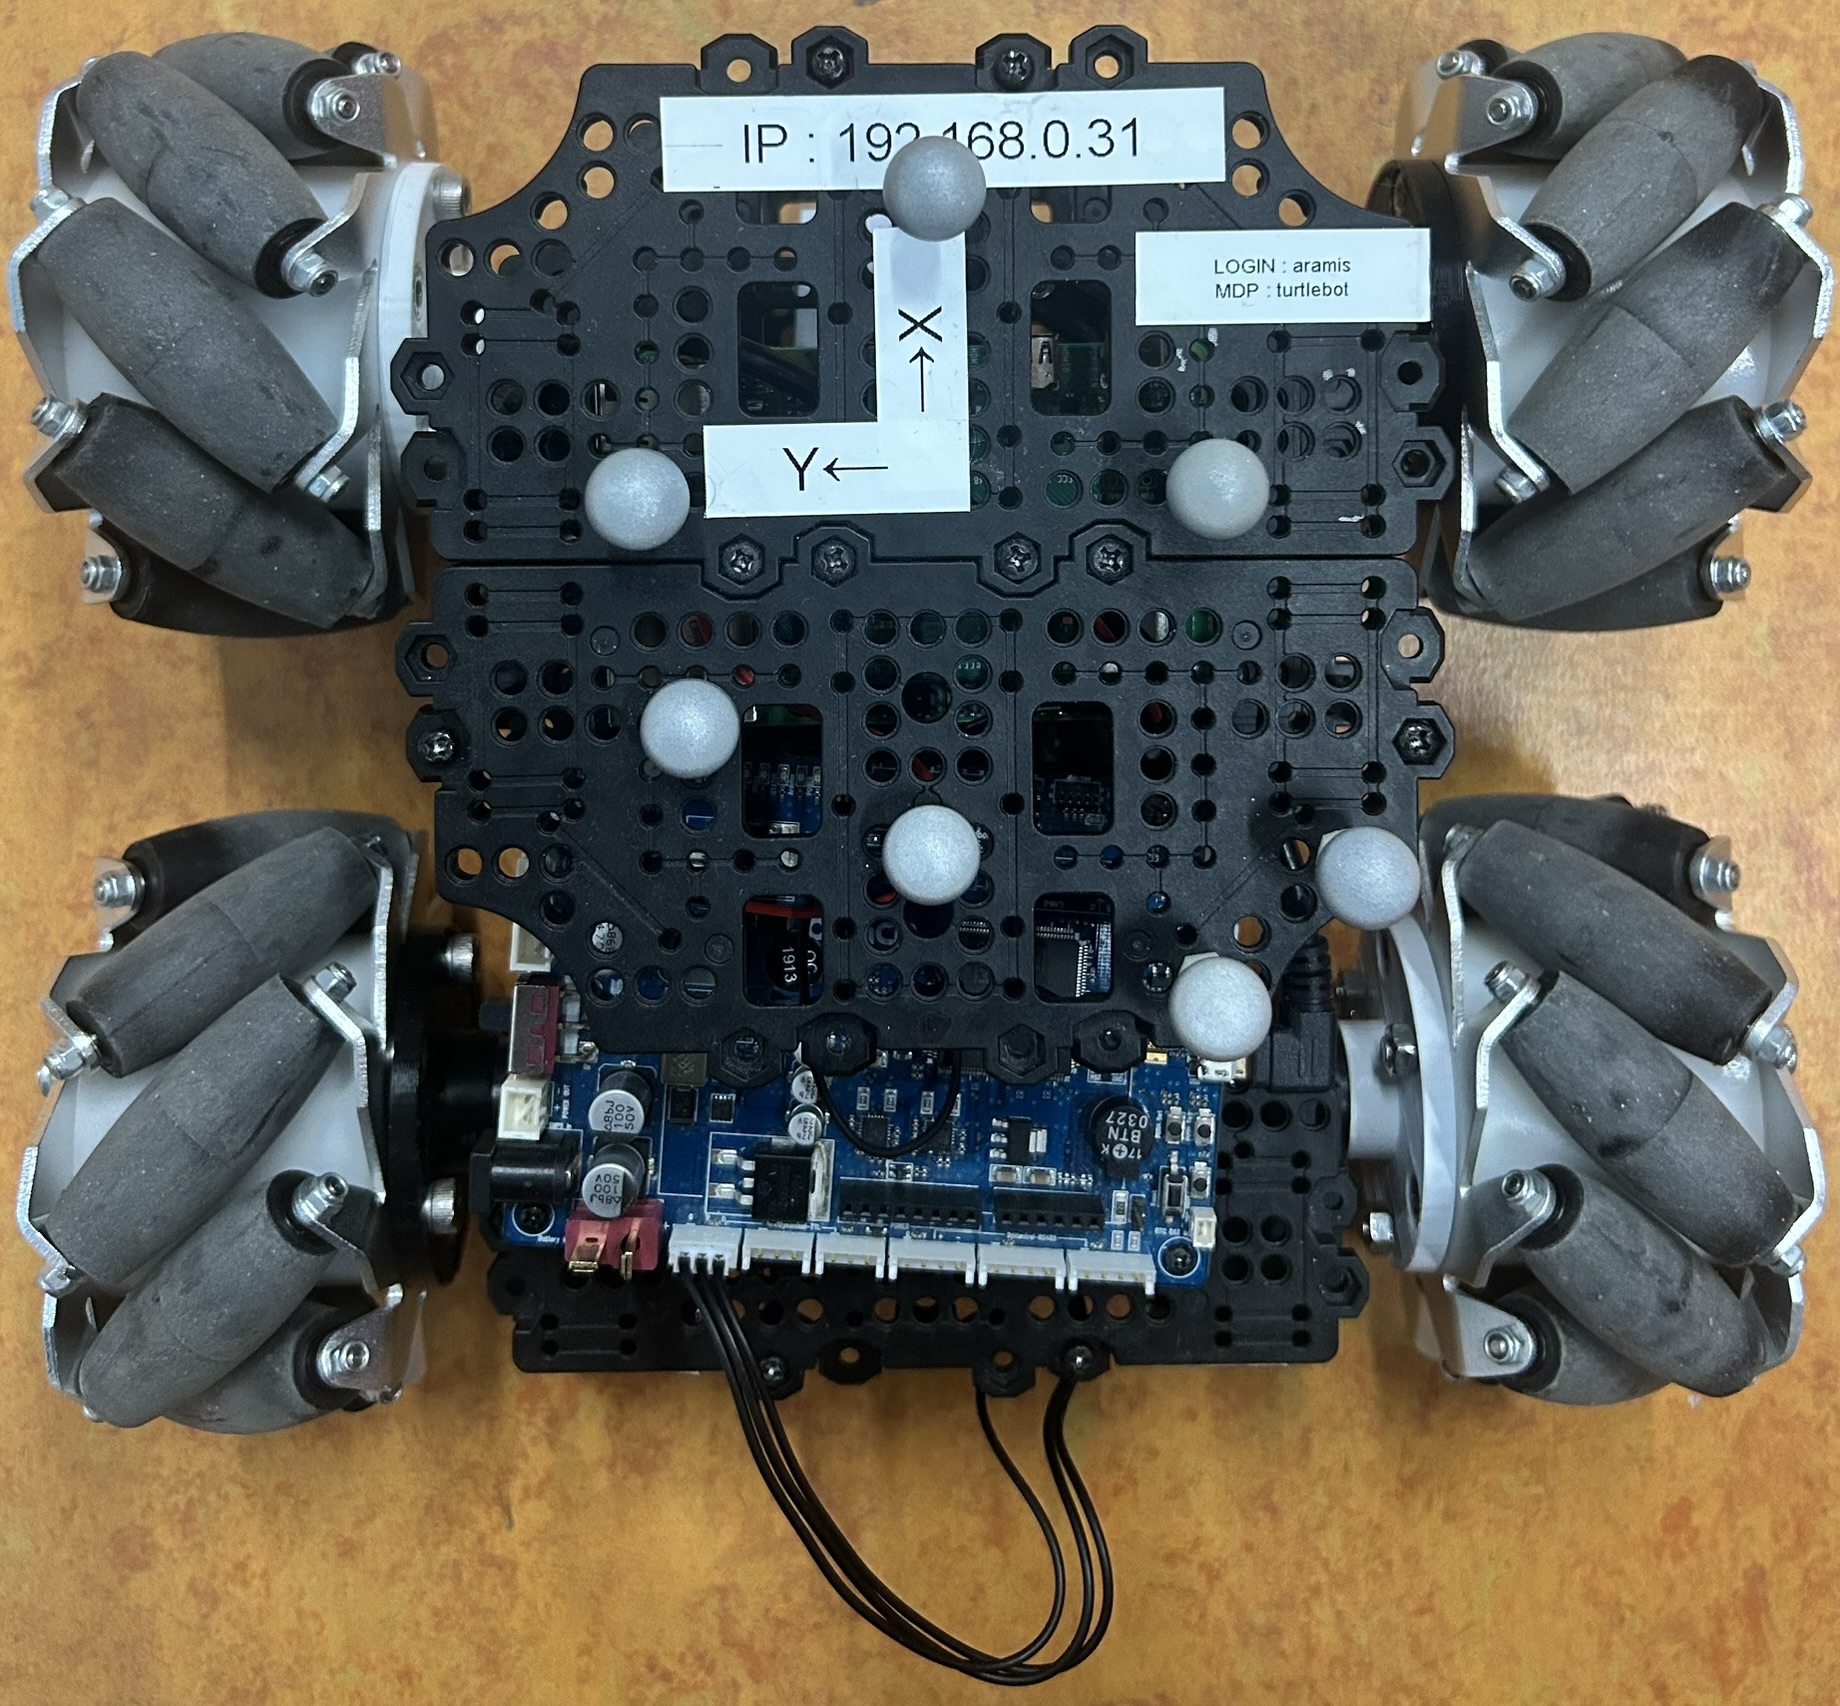
\includegraphics[height=4cm,keepaspectratio]{10-Descriptions_réalisations/Outils/pic/billes.JPEG}
        \caption{Billes de motion capture sur Aramis}
    \end{subfigure}
    \hfill
    %\hspace*{-6cm}% ajuster la valeur (ex: -5mm à -15mm) pour décaler la 2e image vers la gauche
    \begin{subfigure}[t]{0.49\textwidth}
        \centering
        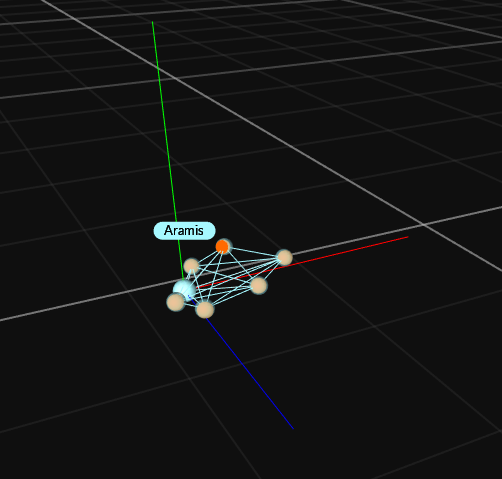
\includegraphics[height=4cm,keepaspectratio]{10-Descriptions_réalisations/Outils/pic/aramis.PNG}
        \caption{Rigid Body d'Aramis dans Motive}
    \end{subfigure}
\end{figure}
\vspace{-0.2cm}